\chapter{Results and Discussion}
\label{ch:results-discussion}

All four systems, the untouched source text, the heuristic baseline, zero-shot T5-small, and fine-tuned T5-small, were evaluated on the same random sample of 150 sentence pairs drawn from the Cochrane-auto test split. The human-written reference is included in the readability comparison as a point of reference, though overlap, simplification, and semantic similarity scores do not apply to it in the same way, since it is what the other systems are being compared against rather than a system in its own right.

\section{Automatic Metrics}
\label{sec:automatic-results}

\Cref{tab:readability-results} reports the three readability formulas for every system, and \cref{tab:generation-results} reports the overlap, simplification, and semantic similarity metrics for the three systems that produce a genuine rewrite.

\begin{table}[htbp]
    \centering
    \caption{Readability scores by system.}
    \label{tab:readability-results}
    \begin{tabular}{@{}lrrr@{}}
        \toprule
        \textbf{System} & \textbf{Flesch Reading Ease} & \textbf{Flesch-Kincaid Grade} & \textbf{SMOG} \\
        \midrule
        Source (unmodified)        & 26.72 & 14.55 & 15.33 \\
        Reference (human)          & 30.14 & 14.67 & 15.31 \\
        Heuristic baseline         & 29.53 & 14.04 & 14.84 \\
        Zero-shot T5-small         & 20.06 & 15.84 & 16.12 \\
        Fine-tuned T5-small        & 24.52 & 15.10 & 15.79 \\
        \bottomrule
    \end{tabular}
\end{table}

\begin{table}[htbp]
    \centering
    \caption{Overlap, simplification, and semantic similarity scores by system.}
    \label{tab:generation-results}
    \begin{tabular}{@{}lrrrrr@{}}
        \toprule
        \textbf{System} & \textbf{BLEU} & \textbf{ROUGE-1} & \textbf{ROUGE-L} & \textbf{SARI} & \textbf{BERTScore-F1} \\
        \midrule
        Source (unmodified)  & 29.59 & 0.553 & 0.497 & 51.94 & 0.881 \\
        Heuristic baseline   & 28.39 & 0.542 & 0.486 & 48.77 & 0.879 \\
        Zero-shot T5-small   & 19.31 & 0.366 & 0.327 & 36.29 & 0.787 \\
        Fine-tuned T5-small  & 29.81 & 0.561 & 0.505 & 50.50 & 0.885 \\
        \bottomrule
    \end{tabular}
\end{table}

\Cref{fig:metric-comparison} shows the same figures as a set of grouped bar charts, and \cref{fig:sari-vs-bertscore} plots SARI against BERTScore for each system, which makes the trade-off between simplification and meaning preservation easier to see at a glance than a table allows.

\begin{figure}[htbp]
    \centering
    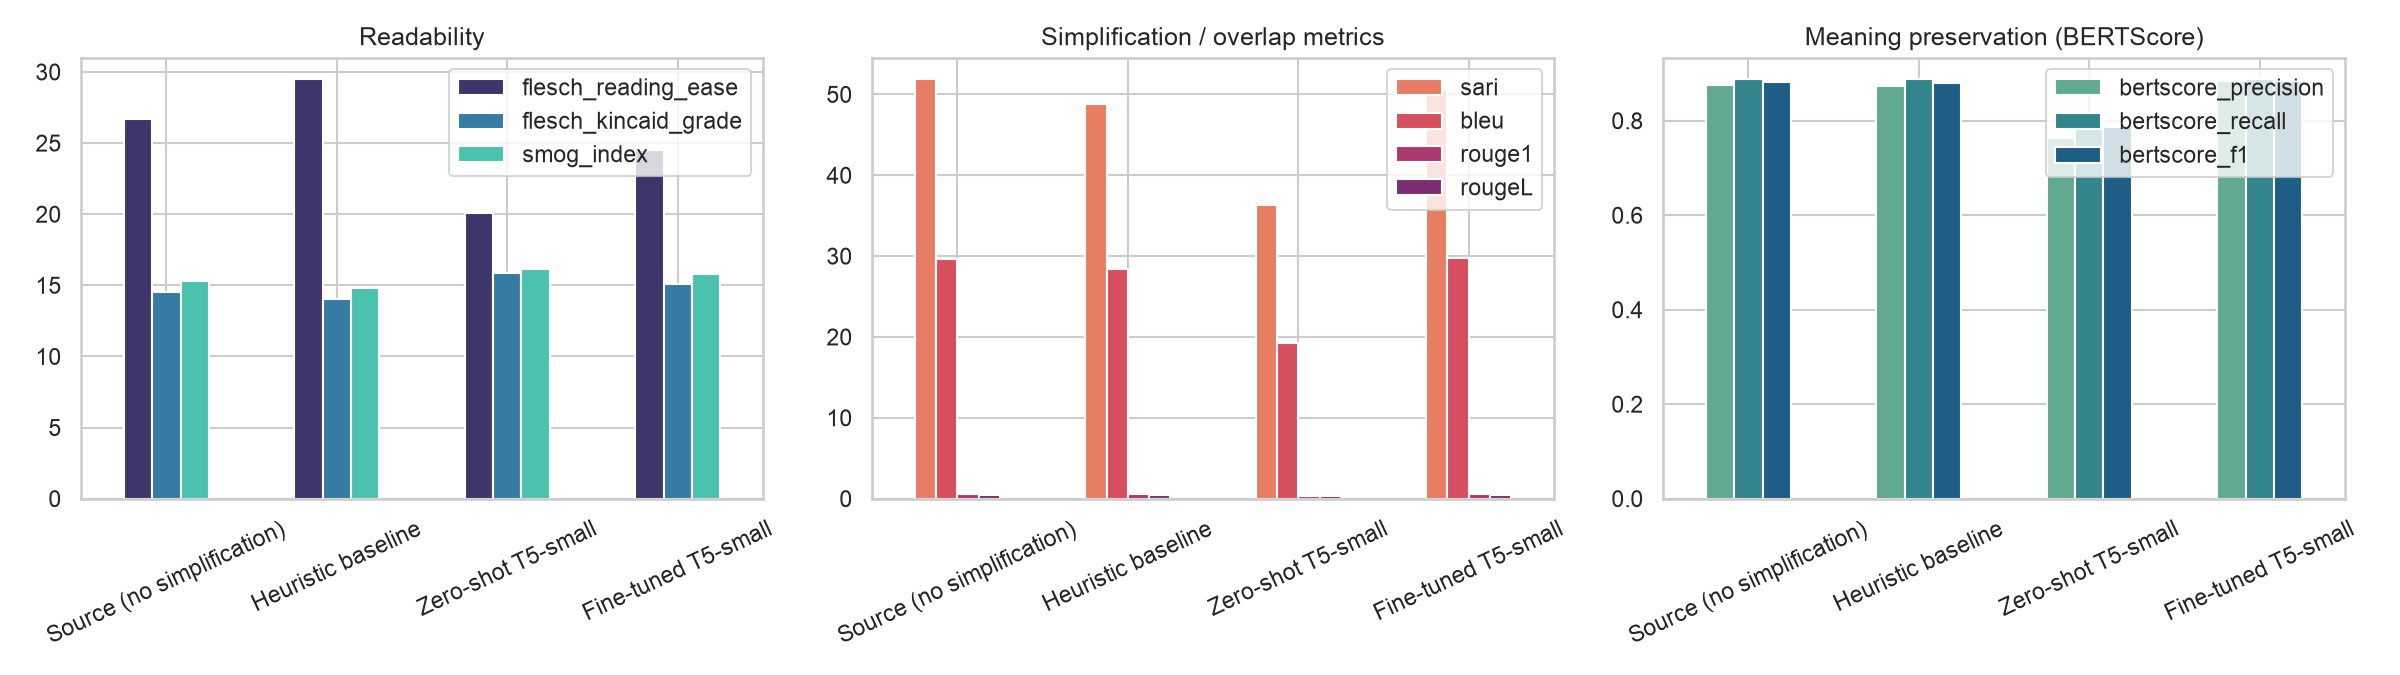
\includegraphics[width=\textwidth]{figures/05_metric_comparison.png}
    \caption{Readability, overlap, simplification, and meaning-preservation metrics across all four systems.}
    \label{fig:metric-comparison}
\end{figure}

\begin{figure}[htbp]
    \centering
    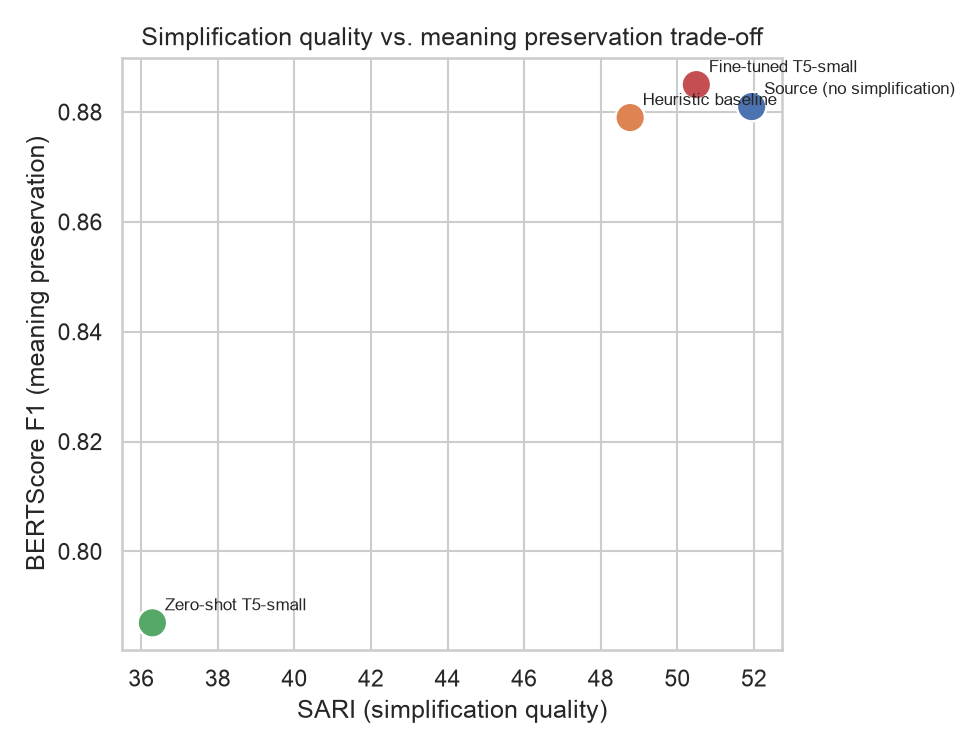
\includegraphics[width=0.75\textwidth]{figures/06_sari_vs_bertscore.png}
    \caption{SARI (simplification quality) against BERTScore F1 (meaning preservation) for each system.}
    \label{fig:sari-vs-bertscore}
\end{figure}

Two results stand out immediately. Fine-tuning made a clear difference relative to the untrained model. Zero-shot T5-small trails every other system on every metric by a wide margin, and a manual reading of its outputs explains why: without any exposure to the \texttt{"simplify: "} task on this data, the model frequently produced disfluent text or switched into a different language entirely rather than simplifying the input. Fine-tuning on only 800 examples for three epochs was enough to eliminate that failure mode completely and bring the model back to fluent, on-task English output.

Against the heuristic baseline, the comparison is closer and more informative. The fine-tuned model edges ahead on BLEU, ROUGE, and BERTScore, and very nearly matches the heuristic baseline's SARI score despite the heuristic system having been designed by hand specifically for this kind of sentence. On the readability formulas, however, the heuristic baseline actually scores slightly better than the fine-tuned model, and both trail the source text's own Flesch Reading Ease by less than might be expected for a system meant to simplify it. This is a genuine and honestly reported finding rather than an oversight, and \cref{sec:qualitative-discussion} explains what a manual reading of the outputs suggests is driving it.

\section{Qualitative Analysis}
\label{sec:qualitative-discussion}

Three examples were selected from the fine-tuned model's outputs on the test sample, one representing a clear success, one representing a partial or ambiguous result, and one representing a genuine failure to simplify. All three are reproduced here in full because the pattern they reveal matters more than any single score.

\subsection*{A Successful Simplification}

\begin{quote}
\textbf{Source:} ``One study with 59 teachers in 43 schools found no significant effects on job-related anxiety (MD -0.25 95\% CI -0.61 to 0.11, very low-quality evidence) or depression (MD -0.26 95\% CI -0.57 to 0.05, very low-quality evidence) after 24 months.''

\textbf{Fine-tuned output:} ``One study with 59 teachers in 43 schools found no significant effects on job-related anxiety or depression after 24 months.''
\end{quote}

The model removed both statistical parentheticals while keeping the claim itself intact and grammatically sound. This is close to the kind of edit the heuristic baseline was designed to make by hand, except the transformer produced it without an explicit rule telling it to strip confidence intervals. It is a genuine example of learned, rather than scripted, simplification behaviour.

\subsection*{A Neutral Case}

\begin{quote}
\textbf{Source:} ``Six RCTs with a total of 1211 participants were eligible; five trials evaluated oral aciclovir, and one, with 419 participants, evaluated oral famciclovir.''

\textbf{Reference:} ``They included a total of 1319 participants.''

\textbf{Fine-tuned output:} ``Six trials with a total of 1211 participants were eligible; five evaluated oral aciclovir, and one, with 419 participants, evaluated oral famciclovir.''
\end{quote}

The model made only a small lexical change here, replacing ``RCTs'' with ``trials,'' while the human reference summarised the same information in a completely different and much shorter way. Notice also that the reference states a participant count, 1{,}319, that does not match the 1{,}211 given in the source sentence. That discrepancy appears to be a genuine inconsistency in the original Cochrane materials rather than a modelling error, and it is a useful reminder that not every gap between a model's output and its reference reflects a failure of simplification. Sometimes it reflects noise already present in the training data, which is worth flagging for anyone extending this work.

\subsection*{A Failure Case}

\begin{quote}
\textbf{Source:} ``We identified only low- or very low-certainty evidence to judge the effectiveness of inhaled antibiotics for the treatment of pulmonary exacerbations in people with cystic fibrosis.''

\textbf{Reference:} ``We graded the certainty of the evidence as very low or low.''

\textbf{Fine-tuned output:} \textit{(identical to the source, no change made)}
\end{quote}

Here the model made no edit at all, while the reference restructures the sentence almost completely, dropping the specific clinical context and restating only the certainty judgement. This is the clearest evidence in the results that, at the training scale used for this confirmation run, the model has learned to make small, local edits such as deleting a clause or swapping a word, but has not yet learned the kind of deeper restructuring a human writer uses when a sentence needs more than light editing. That is a limitation of scale rather than of the approach itself, and \cref{ch:conclusion} discusses what a longer training run on the full dataset would be expected to change.

\section{Discussion}
\label{sec:discussion}

Read together, these results support a specific and fairly narrow conclusion rather than a sweeping one. Fine-tuning a small transformer on domain-specific aligned data clearly teaches it to behave sensibly on this task, where the same model without fine-tuning does not. It also modestly outperforms a hand-built heuristic on the metrics designed specifically for simplification and meaning preservation, SARI and BERTScore, while trailing that same heuristic slightly on surface readability. The most likely explanation, based on the manual reading above, is that this confirmation run's small training set and short schedule taught the model a conservative editing strategy rather than the more substantial restructuring that both the heuristic rules and the human reference summaries sometimes apply. That the heuristic baseline can compete with, and in one respect beat, a fine-tuned transformer is itself a useful finding. It suggests that at least part of what makes Cochrane lay summaries easier to read, removing dense statistical detail, is learnable by hand-written rules almost as well as by a trained model, at least at this scale of training.

This chapter's results also revisit a point raised in \cref{ch:dataset}: a meaningful share of the reference summaries do more than compress their source sentence, sometimes adding context, sometimes restating a different but related fact, and occasionally, as in the aciclovir example above, containing an inconsistency that has nothing to do with simplification quality at all. Any evaluation of this task needs to hold that in mind before treating a lower automatic score as straightforward evidence of a weaker model.
